\chapter{Contexto y Definición del Problema}
% 

\section{Descripción clara del problema a ser resuelto}

Las ciudades modernas generan continuamente grandes cantidades de información georreferenciada como resultado de diversas actividades urbanas, incluyendo reportes de criminalidad, accidentes de tránsito, sistemas de transporte y plataformas digitales basadas en localización \cite{huang2021analytics, ramirez2021sensors, kamrowska2021impact}. El crecimiento sostenido de estas fuentes ha incrementado significativamente la disponibilidad de datos espaciales capaces de describir fenómenos que ocurren sobre el territorio urbano \cite{huang2021analytics, avram2026advancing}. Esta abundancia ha impulsado el desarrollo de metodologías de análisis geoespacial orientadas a comprender patrones espaciales y extraer conocimiento útil. Como consecuencia, el procesamiento eficiente de grandes volúmenes de información geográfica se ha convertido en un componente fundamental para apoyar la planificación urbana y la toma de decisiones basadas en evidencia \cite{huang2021analytics, kamrowska2021impact, avram2026advancing}.

En este contexto, el análisis espacial de eventos urbanos —como la incidencia criminal— exige identificar la ubicación exacta y la frecuencia de los sucesos para descubrir patrones territoriales. El estado del arte demuestra que este análisis se formaliza asignando las coordenadas de los eventos a un grafo espacial que modela la infraestructura vial, dado que las redes urbanas condicionan intrínsecamente la distribución de estos fenómenos \cite{kozhabek2025multi, yap2023urbanity}. Mediante procesos de \textit{Map Matching}, la información cruda se vincula a representaciones topológicas para su evaluación analítica \cite{xue2022quantifying}.

Sin embargo, los grafos urbanos extraídos directamente de bases de datos espaciales abiertas, como OpenStreetMap (OSM), sufren de una excesiva densidad geométrica. Estas redes presentan múltiples aristas paralelas y vértices con conexiones redundantes (necesarias para el trazado de mapas visuales) que no aportan información analítica funcional sobre el evento urbano.

Esta densidad genera un grave problema de \textbf{dilución o dispersión espacial}. Es decir, si se asigna un conjunto de eventos a un grafo crudo, la verdadera densidad del fenómeno se pierde al redistribuirse estadísticamente entre múltiples aristas adyacentes, en lugar de concentrarse en una única vía lógica. 

Como se ejemplifica en la Figura \ref{fig:dilucion_semantica}, al evaluar una avenida con múltiples carriles paralelos, los eventos delictivos pueden distribuirse entre diferentes elementos de la red aun cuando correspondan funcionalmente a una misma vía urbana. Esta situación puede dificultar la identificación de patrones espaciales consistentes y afectar la interpretación de indicadores de densidad o concentración. En consecuencia, surge la necesidad de explorar representaciones alternativas que permitan preservar la estructura vial relevante para el análisis sin introducir distorsiones significativas en la distribución espacial de los eventos.

\begin{figure}[H]
    \centering
    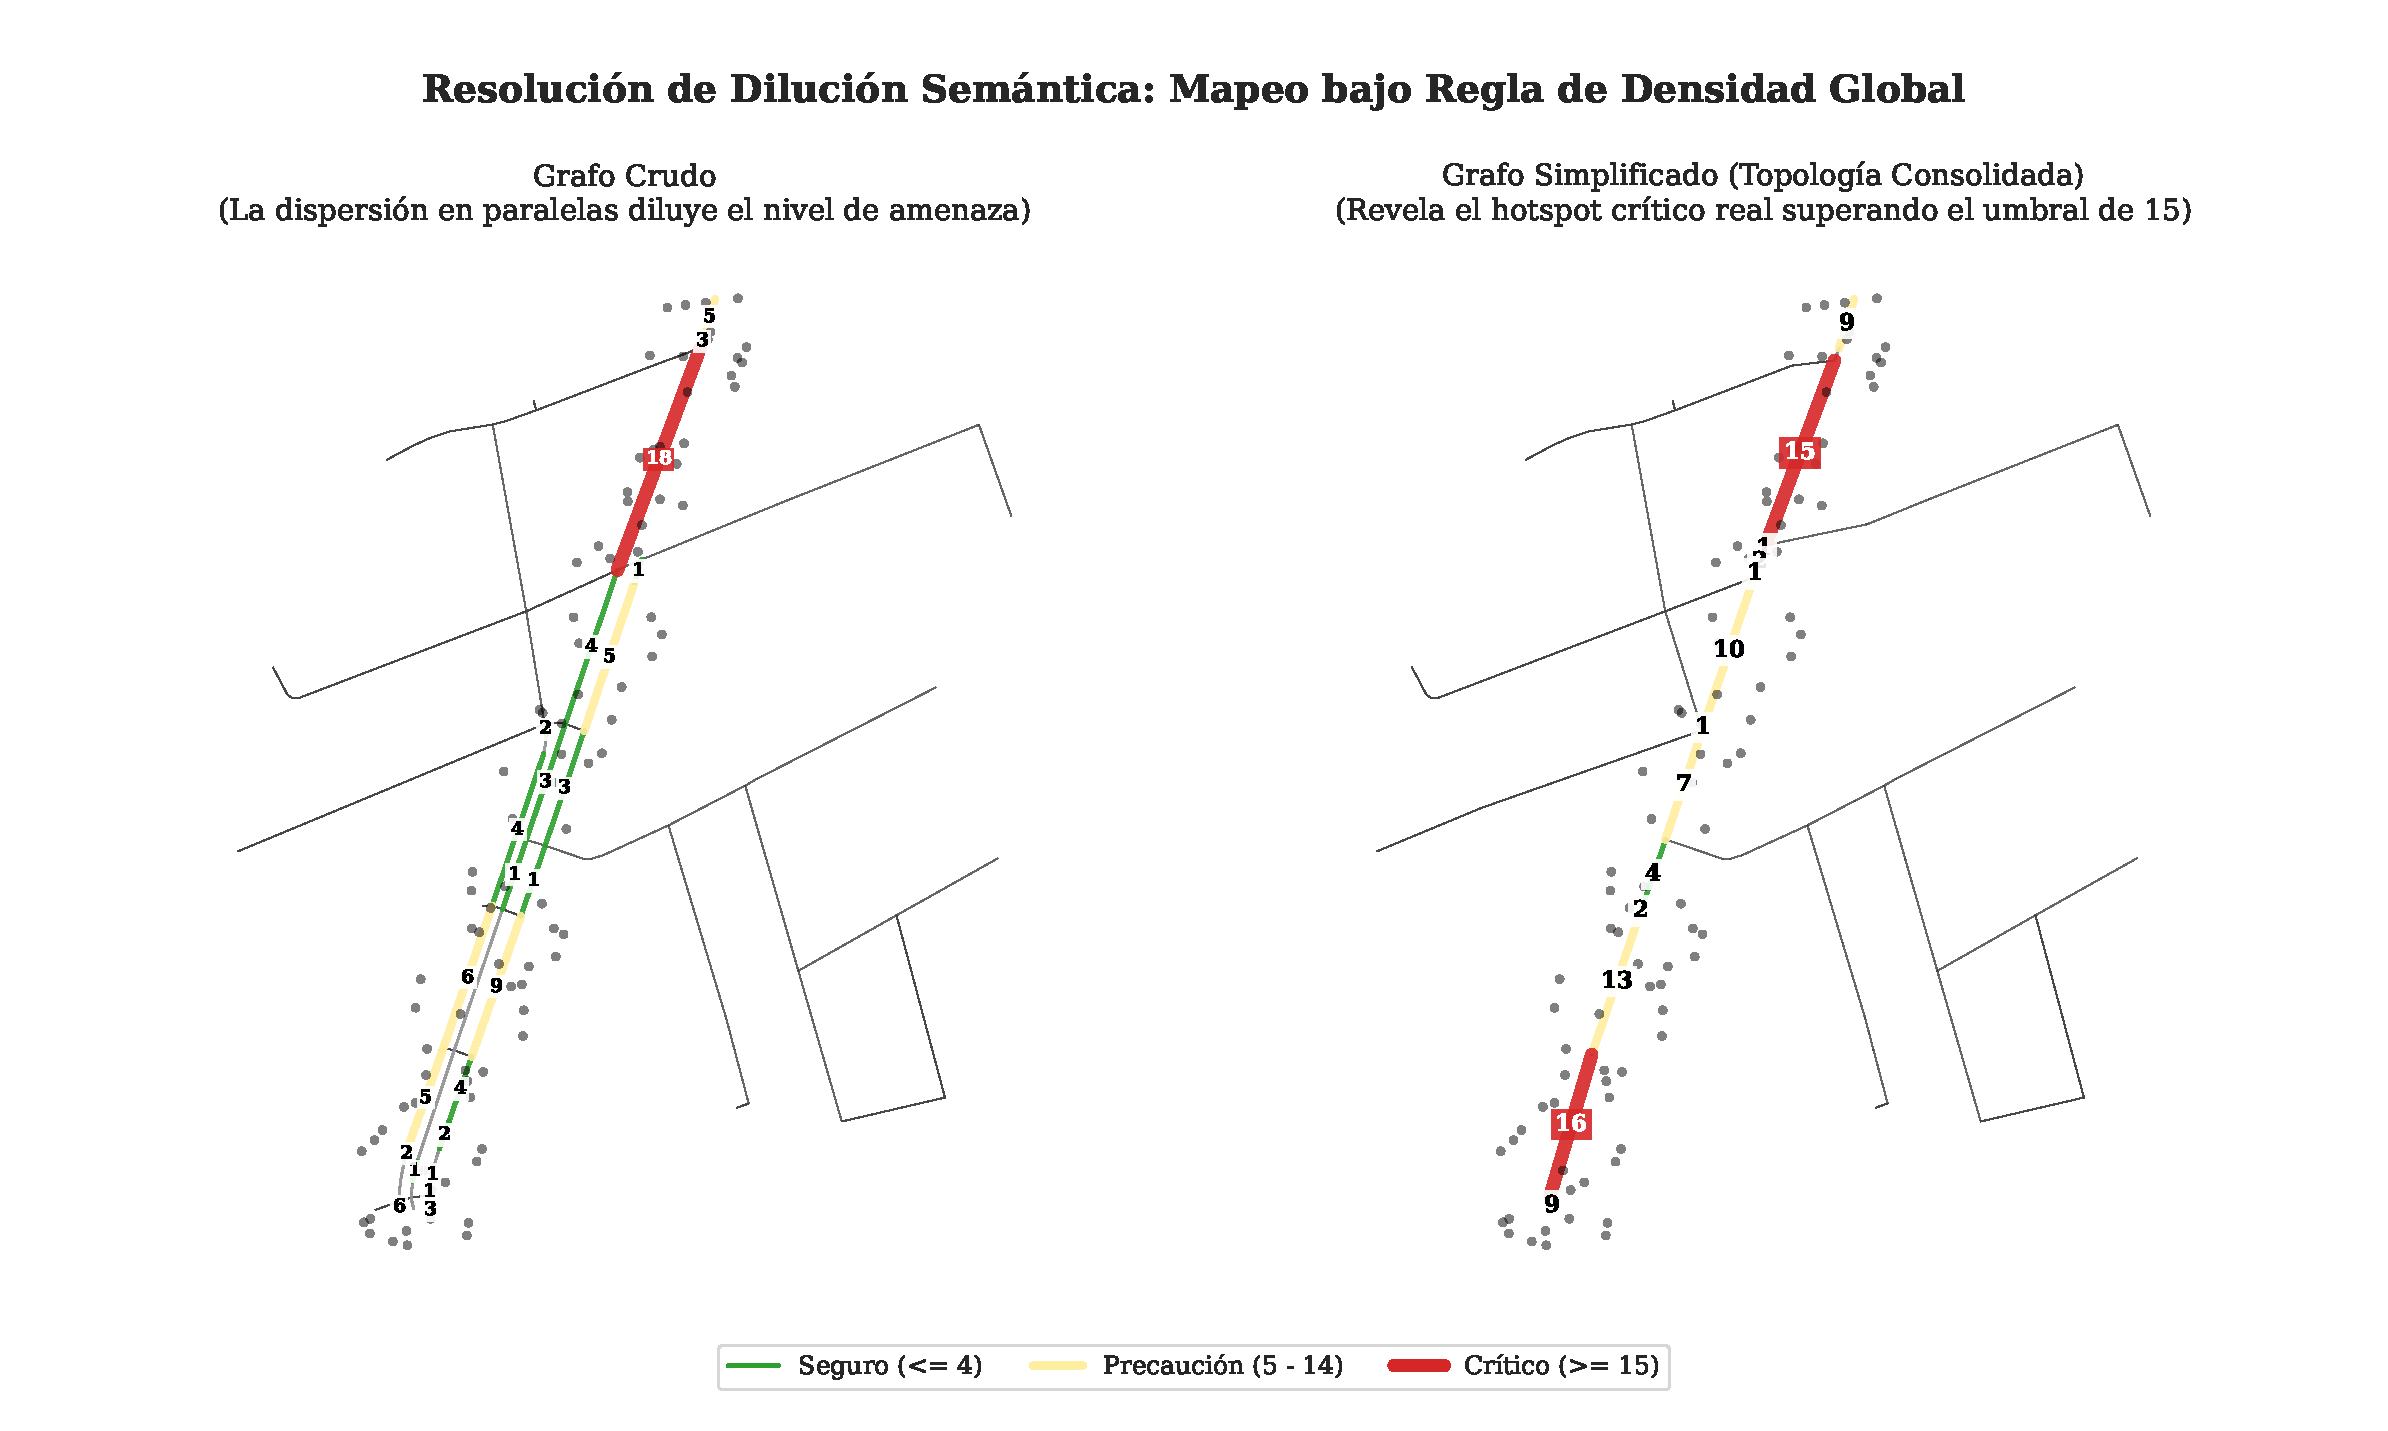
\includegraphics[
        width=\textwidth,
        trim=3.5cm 0cm 3.5cm 0cm,
        clip
    ]{../images/disolucion_semantica.pdf}
    \caption{Impacto de la granularidad topológica en el análisis de densidad espacial. A la izquierda, la red cruda diluye los eventos sobre aristas paralelas, ocultando la amenaza real. A la derecha, el colapso semántico del grafo concentra los eventos sobre la vía lógica, revelando la verdadera magnitud del \textit{hotspot}.}
    \label{fig:dilucion_semantica}
\end{figure}

Si bien existen diversos métodos de simplificación de redes urbanas, gran parte de ellos han sido diseñados con objetivos orientados a la compresión geométrica, la representación cartográfica o la reducción de complejidad estructural. Sin embargo, la influencia de estas transformaciones sobre la distribución espacial de eventos y sobre la preservación de propiedades analíticas relevantes continúa siendo un aspecto que requiere mayor investigación.

Por lo tanto, la pregunta de investigación central es: ¿Cómo simplificar eficientemente un grafo espacial urbano para concentrar la densidad de eventos, garantizando la recuperación de su semántica original sin alterar las invariantes topológicas que definen la ciudad?

\section{Motivación y relevancia (técnica, social, económica)}

La implementación de algoritmos avanzados de simplificación topológica se justifica bajo tres dimensiones fundamentales:

\begin{itemize}
    \item \textbf{Relevancia técnica:} Los algoritmos de ruteo y \textit{Map Matching} estándar sufren una severa sobrecarga de memoria y tiempo de procesamiento cuando operan sobre redes a escala de ciudad. La simplificación geométrica rigurosa proporciona ahorros significativos de memoria (RAM) al reducir la dimensionalidad del grafo $|V| + |E|$. Esto permite diseñar arquitecturas escalables donde las consultas espaciales operan con una rapidez drásticamente mayor, sin sacrificar la semántica analítica del sistema.
    
    \item \textbf{Relevancia social:} Prevenir la dilución espacial es crítico para la seguridad ciudadana. Un mapeo eficiente y concentrado permite a las autoridades identificar y predecir \textit{hotspots} criminales con alta fidelidad, optimizando el diseño de estrategias de prevención y la asignación de rutas de patrullaje.
    
    \item \textbf{Relevancia económica:} Al reducir el peso del modelo espacial y acelerar los tiempos de cómputo, se disminuyen radicalmente los ciclos de CPU y los requerimientos de infraestructura (\textit{Cloud Computing}), abaratando los costos operativos de despliegue para entidades gubernamentales o investigativas.
\end{itemize}

\section{Impacto esperado}

Se proyecta que la arquitectura propuesta genere dos impactos críticos en el análisis de redes urbanas:

\begin{enumerate}
    \item \textbf{Mejora en la eficiencia computacional:} Mediante la reducción de la complejidad estructural de la red y el uso de mecanismos eficientes de indexación espacial, se espera disminuir significativamente los tiempos requeridos para operaciones de asignación espacial y análisis sobre grandes volúmenes de eventos georreferenciados.
    
    \item \textbf{Preservación estricta de la topología y precisión:} La simplificación no debe entenderse como la destrucción de datos, sino como su consolidación. Se espera mantener el error de proyección espacial (bajo el estándar EPSG:3857) cercano a cero. Fundamentalmente, se busca conservar propiedades asociadas a conectividad, navegabilidad y consistencia de rutas, de manera que la red simplificada continúe siendo útil para aplicaciones de análisis espacial.
\end{enumerate}

\section{Formulación de suposiciones e identificación de restricciones}

Para delimitar el alcance del presente trabajo, se establecen las siguientes suposiciones:
\begin{itemize}
    \item Los datos delictivos son entidades discretas y estáticas representadas por coordenadas geográficas bidimensionales.
    
    \item OpenStreetMap (OSM) será utilizado como fuente cartográfica de referencia debido a su amplia adopción en investigaciones de análisis espacial, movilidad urbana y redes de transporte.

    \item \textbf{Inferencia Semántica:} Se asume que la semántica topológica de una red urbana no puede inferirse puramente a través de métodos geométricos abstractos (como distancias euclidianas). Para una simplificación correcta, es imperativo \textit{recuperar} la semántica inyectando información auxiliar extraída del dominio del grafo (tales como nombres de vías, tipos de \textit{highway} y jerarquía de conexión).
\end{itemize}

Asimismo, se identifican las siguientes restricciones en el diseño experimental:
\begin{itemize}
    \item El análisis se efectuará sobre un modelo de red estático, excluyendo variables de fricción dinámica como velocidades en tiempo real o densidades de tráfico fluctuantes.
    \item El alcance computacional se concentra exclusivamente en las fases de preprocesamiento, simplificación topológica estructurada y la asignación espacial de puntos estáticos.
\end{itemize}